\documentclass[tikz,border=5pt]{standalone}
\usepackage{tikz}
\usepackage{pgfplots}
\pgfplotsset{compat=1.18}

\begin{document}

% Breit-Wigner Resonance Curve
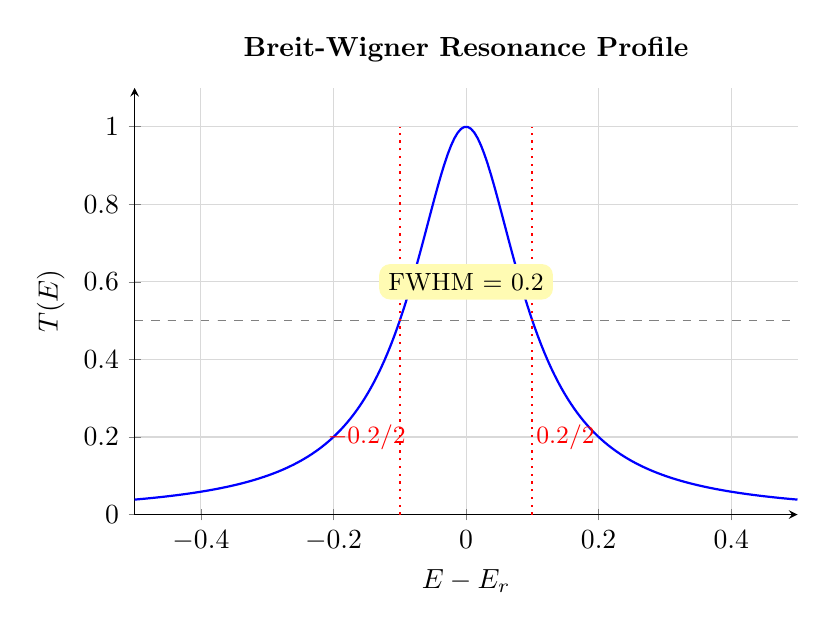
\begin{tikzpicture}
\begin{axis}[
    width=10cm,
    height=7cm,
    xlabel={$E - E_r$},
    ylabel={$T(E)$},
    title={\textbf{Breit-Wigner Resonance Profile}},
    xmin=-0.5, xmax=0.5,
    ymin=0, ymax=1.1,
    axis lines=left,
    grid=major,
    grid style={gray!30},
    samples=200,
]

% Parameters
\def\Gamma{0.2}

% Breit-Wigner function
\addplot[thick,blue,domain=-0.5:0.5] 
    {((\Gamma)^2/4)/(x^2 + (\Gamma)^2/4)};

% Half maximum line
\addplot[gray,dashed,domain=-0.5:0.5] {0.5};

% Gamma/2 markers
\addplot[red,dotted,thick] coordinates {(0.1,0) (0.1,1)};
\addplot[red,dotted,thick] coordinates {(-0.1,0) (-0.1,1)};

% Annotations
\node[fill=yellow!30,rounded corners,font=\small] at (axis cs:0,0.6) {FWHM = $\Gamma$};
\node[font=\small,red] at (axis cs:0.15,0.2) {$\Gamma/2$};
\node[font=\small,red] at (axis cs:-0.15,0.2) {$-\Gamma/2$};

\end{axis}
\end{tikzpicture}

\end{document}
